\chapter{Экспериментальная часть}

В данном разделе будет произведено сравнение вышеизложенных алгоритмов.

\section{Временные характеристики}


Для сравнения возьмем квадратные матрицы размерностью [10, 20, 30,\dots,100]. 
Так как подсчет умножения матриц считается короткой задачей, воспользуемся усреднением массового эксперимента. 
Для этого сложим результат работы алгоритма n раз (n >= 10), после чего поделим на n. 
Тем самым получим достаточно точные характеристики времени. 
Сравнение произведем при n = 50.
Результат можно увидеть на рис. \ref{fg:ref3}. 

\begin{figure}[ht!]
	\centering{
		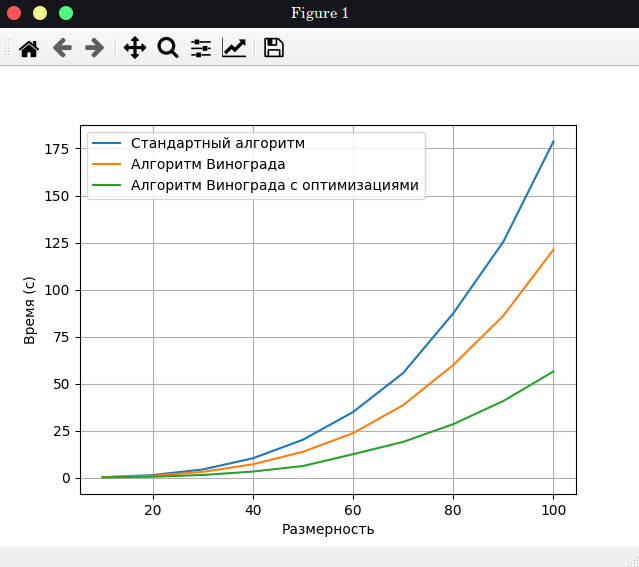
\includegraphics[width=0.8\textwidth]{img/time1.png}
		\caption{Временные характеристики на четных размерах матриц}
		\label{fg:ref3}}
\end{figure}

На рис. \ref{fg:ref4} показана работа алгоритмов с матрицами, размерностью [11, 21, 31,\dots,91].

\begin{figure}[ht!]
	\centering{
		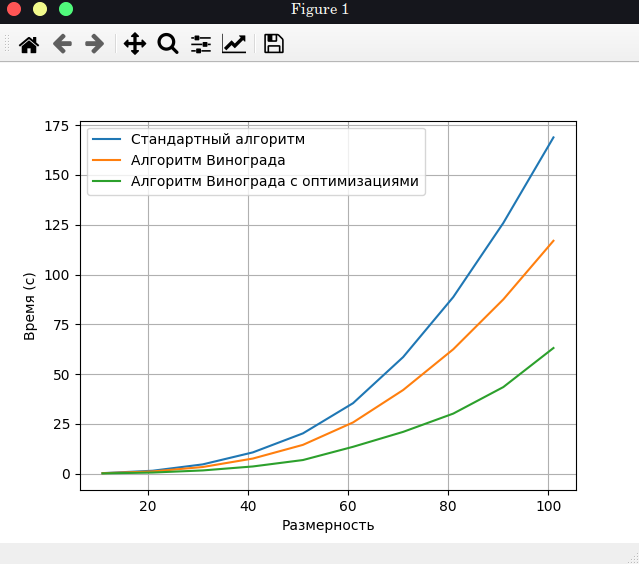
\includegraphics[width=0.8\textwidth]{img/time2.png}
		\caption{Временные характеристики на нечетных размерах матриц}
		\label{fg:ref4}}
\end{figure}

\section{Сравнительный анализ алгоритмов}

\section{Вывод}

В данном разделе было произведено сравнение количества затраченного вре­мени вышеизложенных алгоритмов.
Самым быстрым оказался модифицированный алгоритм Винограда.